\section{End of Chains}
\label{sec:arch.end}

\hl{Thus far, the chapter only covered the parameter regions at the beginning and in the middle of chains.}
This section \hl{investigates} how the chains develop \hl{for larger values of $\beta$}.

\begin{figure}
	\centering
	\subfloat[Larger values for $\beta$]{
		\includegraphics[width=.45 \textwidth]{61_MinimalRepr_Halved/2D_Period_Chain_Ends/result.png}
		\label{fig:arch.chainend.1}
	}
	\subfloat[Even larger values for $\beta$]{
		\includegraphics[width=.45 \textwidth]{61_MinimalRepr_Halved/2D_Period_Chain_Ends_Cont/result.png}
		\label{fig:arch.chainend.2}
	}
	\caption[2D scans of periods in the archetypal model showing the end of the chains]{
		2D scans of periods in the adjusted archetypal model showing the end of the chains of the same period.
		(a) shows the 2D scan for larger values of $\beta$ where ``type B'' regions start missing from the chain of period $16$.
		(b) shows the 2D scan for even larger values of $\beta$ where the chain is no longer connected.
	}
\end{figure}

\Cref{fig:arch.chainend.1} shows a 2D scan of the periods of the \hl{halved} archetypal model where the ``type B'' parameter regions in the chains are visible.
We can see that the ``type B'' parameter region \hl{in} \Cref{fig:arch.chainend.1} between the ``type A'' parameter region marked with point $I_{16}$ and the ``type A'' parameter region marked with point $K_{16}$ is missing.
There should have been the parameter region $\P_{\A^3\B^5\C^2\D^6, \A^2\B^6\C^3\B^5}$ according to the rules laid out in \Cref{sec:arch.dynamics}.

Furthermore, the chain is completely disconnected when looking at even higher values of $\beta$.
\Cref{fig:arch.chainend.2} shows this.
The parameter region $\P_{\A\B^7\C\D^7}$ marked with $M_{16}$ \hl{in} \Cref{fig:arch.chainend.2} is the predicted last ``type A'' parameter region of the chain with period $16$.
It is not connected to the second last parameter region $\P_{\A^2\B^6\C^2\D^6}$ marked with $K_{16}$ \hl{in} \Cref{fig:arch.chainend.2}.

This violates the rules and our expectation for the archetypal model.
\Citeauthor{akyuz2022} observed the same behavior in the original model in \cite{akyuz2022}.
He also looked at a chain of parameter regions with period $16$.
The chain behaved according to the rules up to the second last ``type A'' parameter region, $\P_{\A^2\B^6\C^2\D^6}$.
His hypothesis is that the scan of the periods done here is a two-dimensional one, while the model has more dimensions.
So choosing a different parameter plane for the 2D scan of the periods might reveal a perfect chain with period $16$~\cite{akyuz2022}.
This could also be the case here, since the archetypal model has $5$ parameters and the period scan is done in two dimensions also.
\hl{
	Two ways, one could perhaps obtain such complete chins are introduced next.
}

\hl{
	First, one could adjust the parameters $\alpha$ and $\beta$ to act differently for the values at the end of the chains.
	For example, the parameter $\beta$ influences the parameter $c_L$ directly in the archetypal model.
	But it could also influence some other parameters of the model when $\beta$ crosses some threshold.
	The same can be done for $\alpha$.
}

\hl{
	Secondly, one could try to force the model to behave in such a way, that the shape of the model function at some parameter values $\alpha_2$ and $\beta_2$ is the same as the shape of the model function at the parameter values $\alpha_1$ and $\beta_1$ shifted by $\frac{1}{4}$ where the parameter values $\alpha_1$ and $\beta_1$ belong to a parameter region at the start of a chain.
}
\hl{This can be expressed more precisely using} \Cref{equ:arch.dyn.shift}.
\begin{align}
	f_{\alpha_1, \beta_1}\left(x + \frac{1}{4}\right) & \equiv f_{\alpha_2, \beta_2}(x) \mod 1
	\label{equ:arch.dyn.shift}
\end{align}
\hl{
	This way, the stable cycle at the parameter values $\alpha_2$ and $\beta_2$ is $\Cycle{\A^{m-1}\B\C^{m-1}\D}$, provided the cycle at the beginning of the chain with parameter value $\alpha_1$ and $\beta_1$ is $\Cycle{\A\B^{m-1}\C\D^{m-1}}$.
	The newly chosen parameters should still act similar to the parameters $\alpha$ and $\beta$ in the archetypal model.
}
\hl{More specifically, the new parameter $\alpha$ needs to still have the same effect as in the archetypal model, but also the inverse effect of $\beta$ in the arcehtypal model to achieve the symmetry} \Cref{equ:arch.dyn.shift}.
\hl{
	The same is true for the new parameter $\beta$.
	Also, the model needs to have four quadratic branches.
}
\hl{This is therefore not possible with the archetypal model proposed in this thesis but can be achieved with the piecewise-quadratic model introduced in} \Cref{sec:setup.quad}.
